%\todofilebegin{040\_evaluation\_validation.tex}
%%%%%%%%%%%%%%%%%%%%%%%%%%%%%%%%%%%%%%%%%%%%%%%%%%%%%%%%%%%%%%%%%%%%%%%%%%%%%%
%%%%%%%%%%%%%%%%%%%%%%%%%%%%%%%%%%%%%%%%%%%%%%%%%%%%%%%%%%%%%%%%%%%%%%%%%%%%%%
%%%%%%%%%%%%%%%%%%%%%%%%%%%%%%%%%%%%%%%%%%%%%%%%%%%%%%%%%%%%%%%%%%%%%%%%%%%%%%

\section{Evaluation and Validation}

%%%%%
SOSflow is a large, complex, and completely new tool framework.
%
The core library components comprise more than 12,000 lines of
original C99 code.
%
SOSflow's code base has \textit{not} been systematically optimized for
this pre-release research work -- since it is an open source project,
volunteers are always welcome!
%
It is likely that the observed performance of SOSflow will
dramatically improve with several iterations of focused overhead and
latency refactoring.
%
Many of the behavioral characteristics of SOSflow are the product of
its internal parameters and the configuration of its runtime
deployment, rather than products of its data model and algorithms.
%
The exploration of optimal settings in that combined parameter space
is left for future work: For now the effort was made to select
reasonable default SOSflow configuration parameters and
typical/non-priviledged cluster queues and topologies.
%%%%%

%%%%%
SOSflow as a tool is \textit{production capable} for the purpose of
validating the SOS workflow performance model.
%
As we demonstrate, even the current un-optimized code is able to scale
out to reasonable allocation sizes and handle relatively impressive
varieties, quantities, and rates of data flow.
%
Because of the lack of focused tuning to its internal mechanics and
the general novelty of the architecture, the results and figures
presented here should be considered the \textit{worst-case scenario}
for the performance of SOSflow itself, now and for the future.
%%%%%

%-----------------------------------------------------------------------------
\subsection{Testing Platform and SOS Configurations}

%%%%%
All results were obtained by either probing (figure~\ref{probe_json})
the daemon or by running queries against the SOSflow databases, such
as the one in figure~\ref{example_query}.
%%%%%

%%%%%
\begin{figure}[!t]
  \centering
  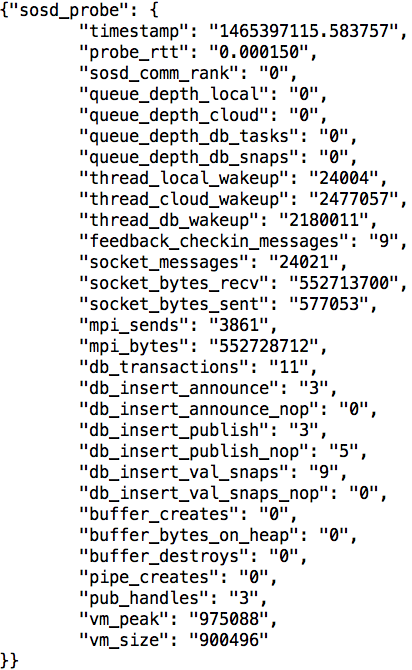
\includegraphics[width=2.5in]{images/probe_json_example.png}
  \caption{JSON Object Returned by SOS's Probe Tool}
  \label{probe_json}
\end{figure}
%%%%%

%%%%%
\begin{figure*}[!t]
\centering
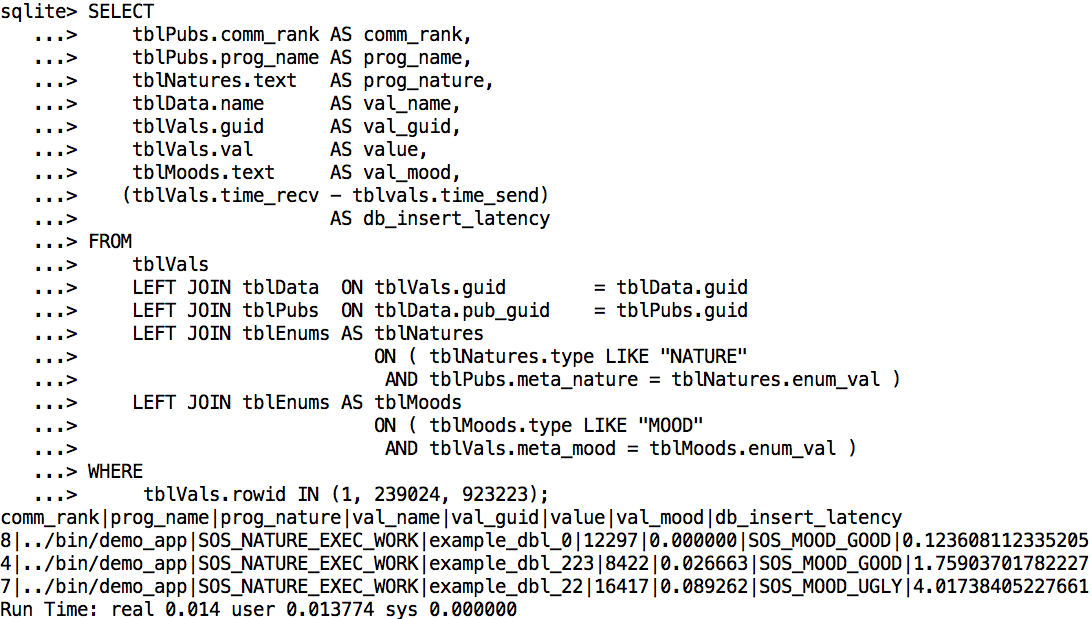
\includegraphics[width=5in]{images/query_example.png}
\caption{Querying the SOSflow Database}
\label{example query}
\end{figure*}
%%%%%

%%%%%
Single node tests of SOSflow used an 8-way Xeon workstation with
Ubuntu linux, gcc, and OpenMPI.
%
Runs were performed by launching the sosd(listener) daemon along with
an sosd(db) instance as background MPI tasks.
%
The demo\_app tool was then also launched as an MPI task with varying
parameters to explore the capabilities of the sosd daemons.
%%%%%

%%%%%
Tests run on the ACISS platform at the University of Oregon were
deployed with the Torque job scheduler as MPICH2 MPI applications at
scales ranging from 3 to 24 nodes, serving 10 demo\_app processes per
node in all cases.
%
The ACISS battery of runs were tuned as stress tests to make ensure
the daemons could operate under reasonably heavy loads.
%
In the 24-node case (figure \ref{aciss_lat_24_agg}) SOSflow processed
72,000,000 values during a 90 second window containing three rounds of
extremely dense API calls.
%%%%%

%%%%%
Real-world use case experiments were conducted on the Cori
supercomputer at The National Energy Research Scientific Computing
Center NERSC.
%
An SOSflow-enabled variant of the Tuning and Analysis
Utilities program (TAUflow) was created as a part of the SOSflow
development work.
%
On Cori, TAUflow was used to instrument the Livermore Unstructured
Lagrangian Explicit Shock Hydrodynamics (LULESH) code.
%
During the execution of LULESH, a thread in TAUflow would periodically
awaken and submit all of TAU's observed performance metrics into the
SOSflow system.
%%%%%

%-----------------------------------------------------------------------------

\subsection{Latency}

%%%%%
When messages are received over the socket by the sosd(listener)
daemon, they are placed in an asynchronous task queue rather than
being handled immediately.
%
This allows the socket reading loop to immediately return to listening
for another connection.
%
There are three threads running inside the daemon that resolve
messages: local\_sync, node\_sync, and db\_sync.
%
The local\_sync thread picks up the incoming messages from the queue
first, unpacks the message and updates the in-memory data
structures.
%
The local\_sync message handler concludes by creating appropriate
tasks in the db\_sync queue to schedule new values for storage, and
then places the original message in the node\_sync queue for
transmission to a sosd(db) aggregator.
%%%%%

%%%%%
The latency figures shown here reveal how long a value is floating in
the asynchronous queues of the daemon before being stored in the
database.
%
Practically speaking this indicates how long it takes after a value is
published before it is available for searching by an analytics module.
%
The in situ latency graphs (figures~\ref{aciss_lat_3_situ} and
\ref{aciss_lat_24_situ}) will be discussed in more detail in the
Scalability section below.
%
Latency in the context of these graphs is \textit{not} the time cost
of calling SOSflow functions: Blocking API calls that message a daemon
over the socket are nearly constant time regardless of daemon load,
also discussed under Scalability.
%%%%%

%%%%%
When a value is inserted into the database the time\_recv field is set,
the time\_pack and time\_sent fields having already been filled by the
original source of the value.
%
Latency is calculated by subtracting the time\_sent from the
time\_recv figures.
%
When a message is migrated from a sosd(listener) instance to a
sosd(db) aggregate daemon, it is packed up together with many other
messages and sent over MPI.
%
On receipt by an sosd(db) role, those composite messages are broken
apart and immediately serviced, causing the db\_sync queue to grow
rapidly in brief bursts as large quantities of data can be arriving
all at once.
%
It is expected that the upper bound on latency for sosd(db) roles will
be higher than the in situ databases.
%%%%%

%%%%%
The asynchronous queues have thread-sequential FIFO ordering, but
because the MPI messages are queued up based on their arrival time,
and a batch is handled competely before the next is processed, there
is no real-time interleaving of database value injections, they are
injected in batches.
%
This creates the sawtooth pattern in figures~\ref{aciss_lat_3_agg} and
\ref{aciss_lat_24_agg}, as the latency for values in the batches near
the bottom of the pile of MPI messages consistently increases until
their batch is injected, detailed in
figure~\ref{aciss_lat_3_agg_detail}.
%%%%%

%%%%%
\begin{figure*}[!t]
\centering
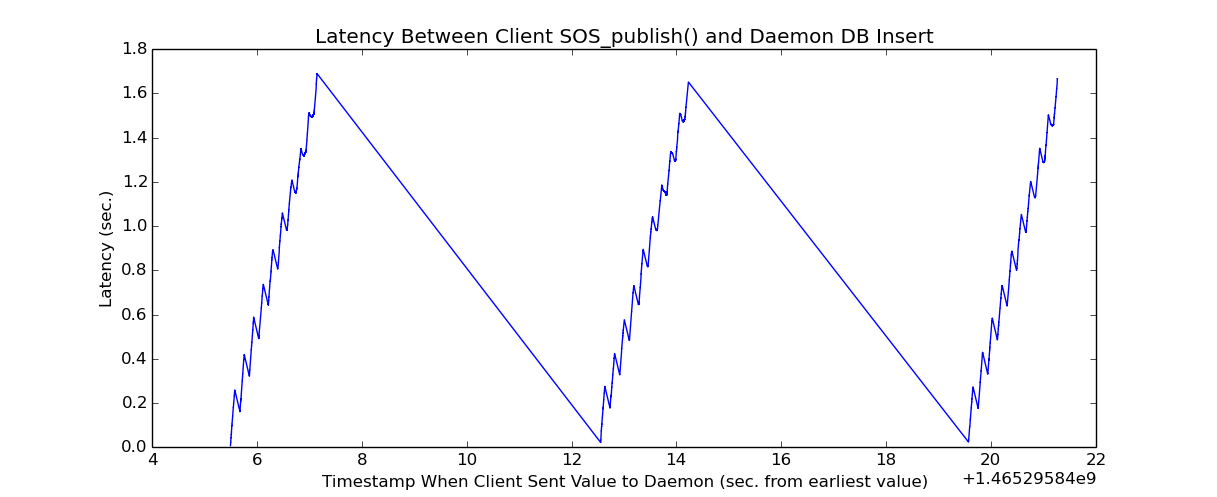
\includegraphics[width=5in]{images/aciss_latency_3_situ.png}
\caption{In Situ Latency (3 Nodes, 30 Applications)}
\label{aciss_lat_3_situ}
\end{figure*}
%%%%%

%%%%%
\begin{figure*}[!t]
\centering
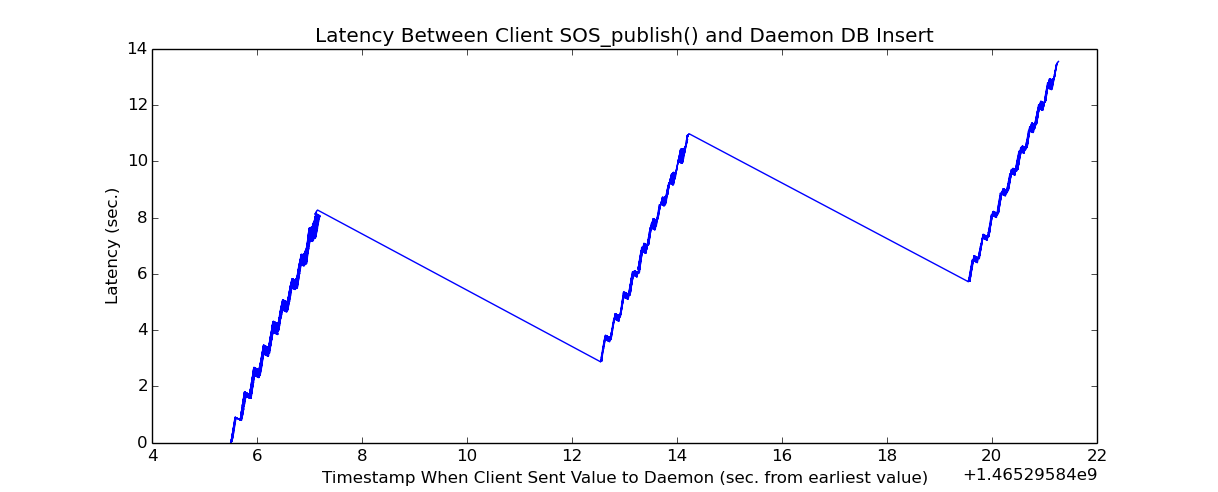
\includegraphics[width=5in]{images/aciss_latency_3_agg.png}
\caption{Aggregate sosd(db) Latency (3 Nodes, 30 Applications)}
\label{aciss_lat_3_agg}
\end{figure*}
%%%%%

%%%%%
\begin{figure*}[!t]
\centering
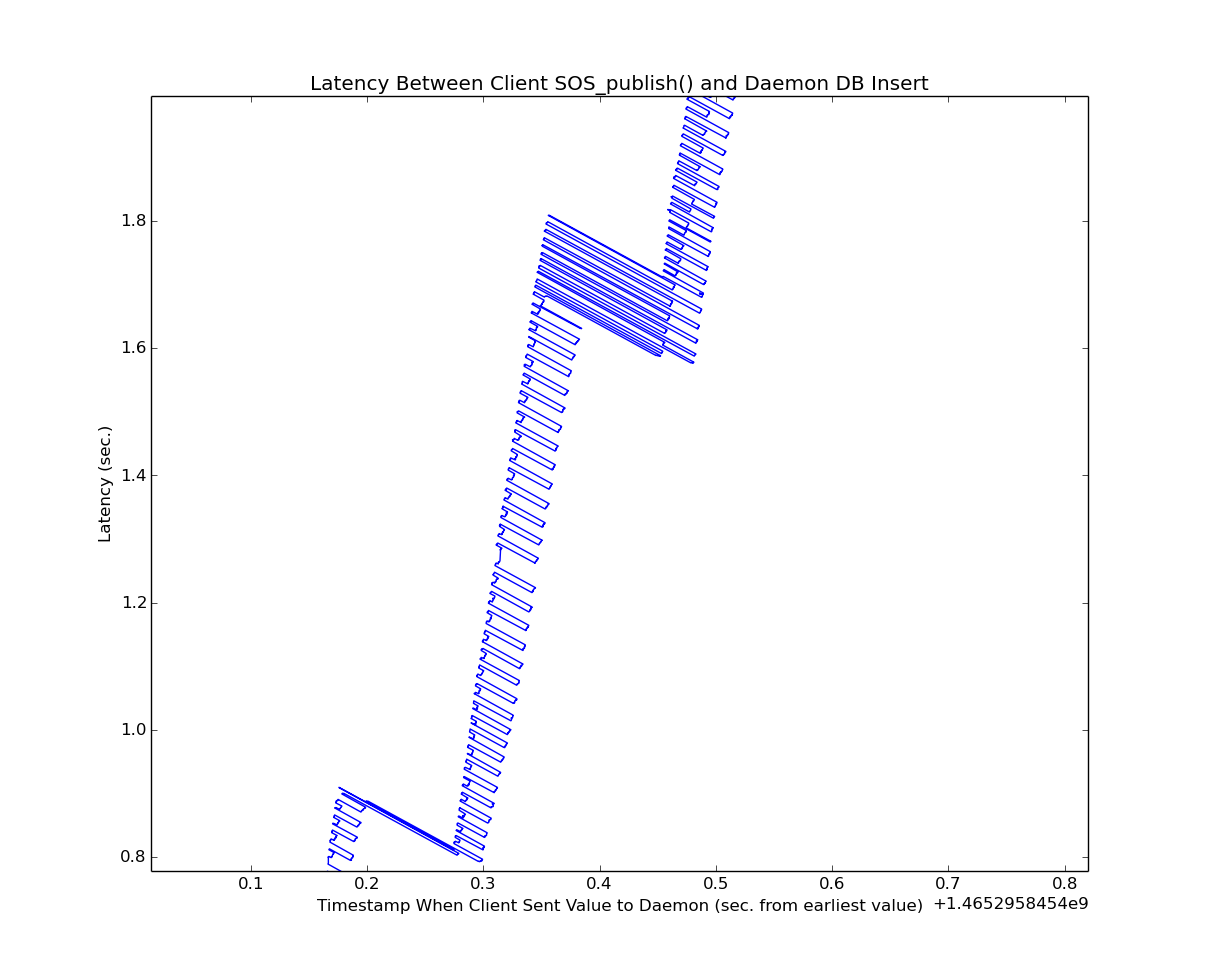
\includegraphics[width=5in]{images/aciss_latency_3_agg_zm.png}
\caption{Aggregate sosd(db) Detail (3 Nodes, 30 Applications)}
\label{aciss_lat_3_agg_detail}
\end{figure*}
%%%%%

%%%%%
\begin{figure*}[!t]
\centering
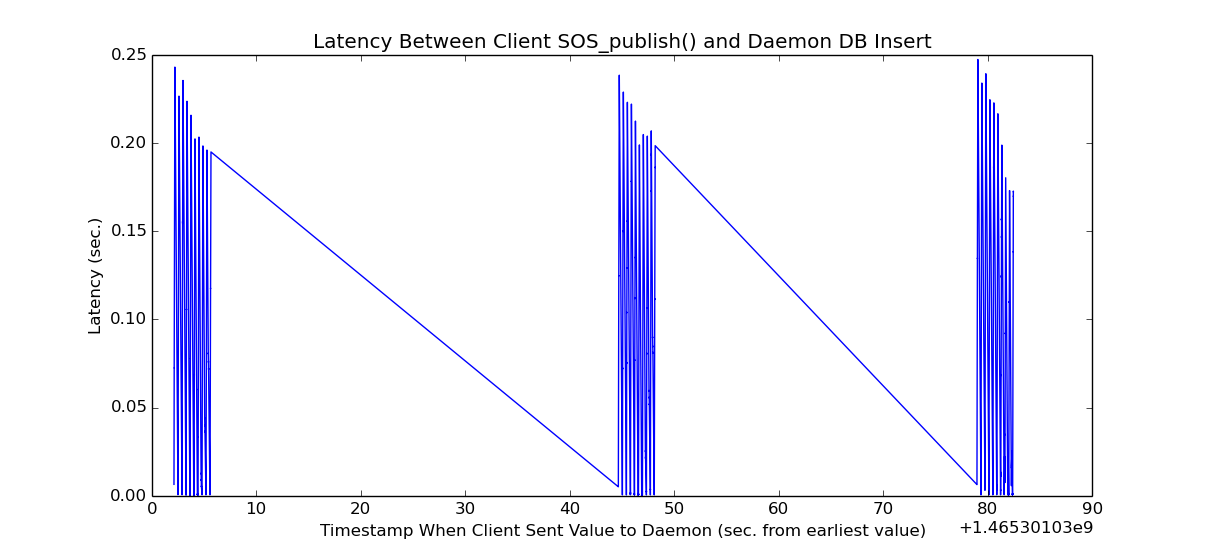
\includegraphics[width=5in]{images/aciss_latency_24_situ.png}
\caption{In Situ Latency (24 Nodes, 240 Applications)}
\label{aciss_lat_24_situ}
\end{figure*}
%%%%%

%%%%%
\begin{figure*}[!t]
\centering
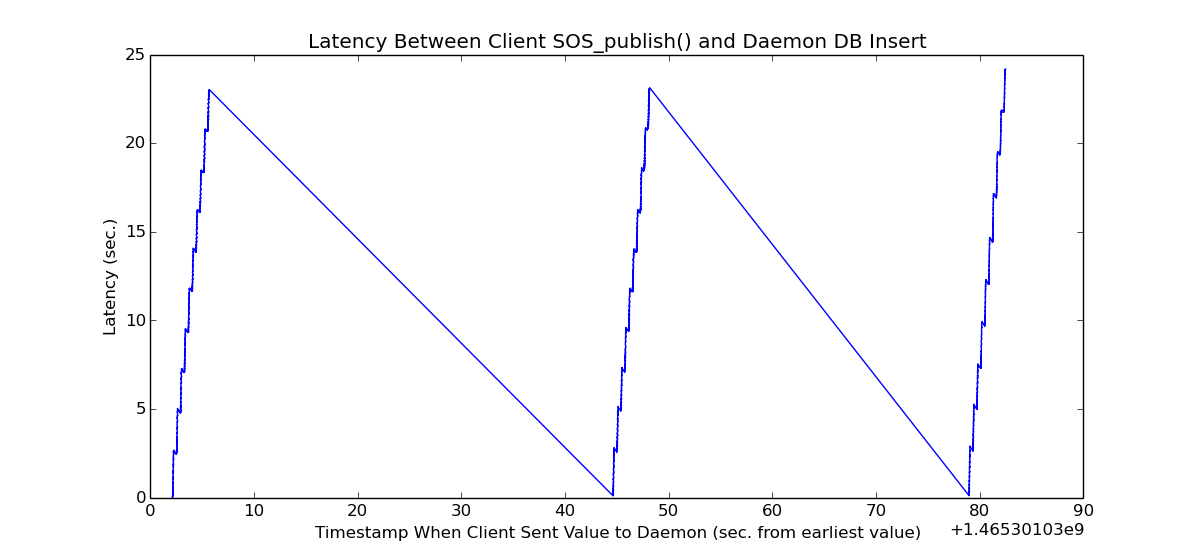
\includegraphics[width=5in]{images/aciss_latency_24_agg.png}
\caption{Aggregate sosd(db) Latency (24 Nodes, 240 Applications)}
\label{aciss_lat_24_agg}
\end{figure*}
%%%%%


%-----------------------------------------------------------------------------

\subsection{Scalability}

%%%%%
SOSflow has a natural scaling fitness for in situ interactivity: As
the size of the allocation for an HPC job increases, the number of
listener daemons increases.
%
In situ interactions with the daemon are nearly constant time
operations regardless of the daemon's workload.
%
This is shown in figures~\ref{sock_cost} and \ref{sock_cost_detail},
where the round trip time (RTT) of a probe message between a client
and the daemon (blue) is projected over a graph of the number of new
messages arriving in a sample window (red).
%%%%%

%%%%%
This information was fetched by sending 9000+ probe messages over a 15
minute window, with a single sosd(listener) rank processing an average
of 43,423 client messages a minute arriving from four different
processes on node.
%
The messages from SOS clients contained more than 14.7 GB of data,
averaging to 338kB per message.
%
Though there are a few spikes in the probe message RTT visible in
figure~\ref{sock_cost}, they are likely not related to SOSflow at all,
as figure~\ref{sock_cost_detail} reveals in detail.
%
The RTT holds steady during low and high volume of traffic from the
other in situ client processes.
%
The mean RTT for the probe messages was 0.003 seconds, and the maximum
RTT was 0.007 seconds.
%
Unlike the SOSflow API calls for publishing data, the probe message is
relatively slow, as the daemon has to immediately service the request
by packaging up a struct of its internal statistics to send back.
%%%%%

%%%%%
\begin{figure*}[!t]
\centering
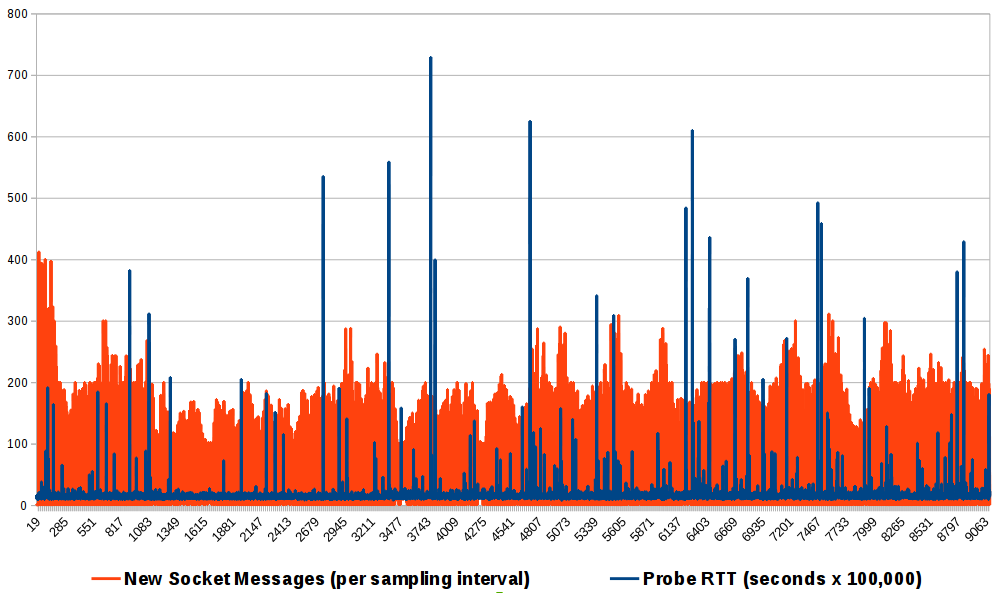
\includegraphics[width=5in]{images/icebox_api_cost_when_slam.png}
\caption{SOSflow Socket Communication Cost (~0.003sec)}
\label{sock_cost}
\end{figure*}
%%%%%

%%%%%
\begin{figure*}[!t]
\centering
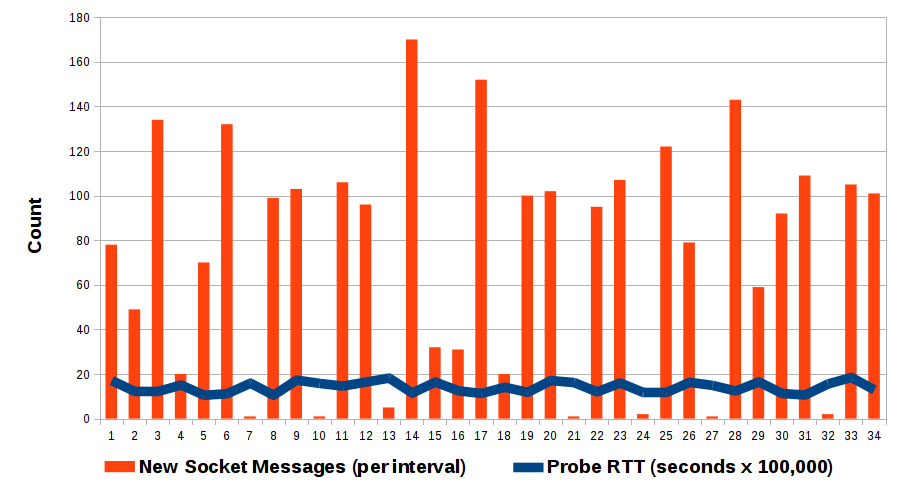
\includegraphics[width=5in]{images/icebox_api_cost_zoom.png}
\caption{SOSflow Socket Communication Cost, Detail}
\label{sock_cost_detail}
\end{figure*}
%%%%%

%%%%%
The data store used by SOS at this time is Sqlite3.
%
It was chosen for its simplicity and essential functionality, and
because its license is open.
%
The configuration for these experiments has Sqlite3 creating a file
and writing to it, rather than representing the database only in RAM
-- though /dev/shm memory-mapped folders are used as the working
directory for the data store wherever possible.
%
For reasonable rates of data injection, Sqlite3 serves the project
well, but at larger scales it is expected that it will be replaced
with a more robust data store.
%
When the rate of value injection into SOSflow exceeds the rate at
which it is able to spool the data into the database, the queues will
fill up to the point where the only option is to discard data or
crash.
%
For the ancitipated use cases that SOSflow is targeting, this should
not be the case, but for stress tests and synthetic demos it is
certainly possible to trigger.
%%%%%

%%%%%
Precursors to this failure case can be seen in the difference between
figures~\ref{aciss_lat_3_situ} and \ref{aciss_lat_24_situ}.
%
In both cases there were 10 processes, each sending 10,000 values to
the sosd(listener) before pausing.
%
In \ref{aciss_lat_3_situ} the 10 processes pause for 0.1 seconds, and
in \ref{aciss_lat_24_situ} they pause for 0.3 seconds.
%
The slightly longer pause completely changes the shape of the latency
graph, and dramatically cuts down on the upper bound for the time a
value stayed in the asynchronous queues of the in situ daemon,
bringing it from 1.8 seconds down to 0.25 seconds.
%
The queues were able to fully drain with the 0.3 seconds pause,
whereas the 0.1 second delay gives rise to the ascending sawtooth
pattern more typical of sosd(db) ranks dealing with bundles of
messages coming in from MPI.
%%%%%

%%%%%
In the case of the in situ communication, the sawtooth shape is purely
a function of publishing in data faster than it can be written out to
the database store.
%
In the aggregate case the sawtooth is a product of data having been
generated and timestamped simultaneously across the cluster, then
being secondarily injected in an aggregate database in a
linear-per-node order of MPI message arrival.
%
The aggregator does not open all pending messages to interleave
individual values, though there will likely be refactoring to provide
more fair sharing of latency across finer grained units.
%%%%%

%%%%%
To avoid excessive queue depth and resource consumption, it is
important to ensure natural pauses exist after periods of dense value
injection so that daemon queues can flush.
%
Future work on SOSflow will add mechanisms to automatically throttle
value intake when this behavior is detected in order to increase the
robustness of the daemons.
%%%%%


%%%%%
SOSflow is configured at launch with a set number of aggregator
databases.
%
The validation tests on ACISS used 3 sosd(db) instances to divide up
the workload, while the TAUflow + LULESH experiments on Cori used a
single aggregator.
%
As many instances of aggregators can be spawned as needed in order to
support the quantity of data being injected from a global
perspective.
%
Because all data is tagged with a GUID, these databases can be
concatenated after the run concludes without collision of identities
wiping out unique references.
%%%%%


%-----------------------------------------------------------------------------

\subsection{Overhead and Perturbation}

%%%%%
Synthetic stress test experiments do not give the best picture of the
overhead and perturbation of real-world applications.
%
In more realistic examples SOSflow's presence and activity in situ
resulted in just over 1\% percent increase in the execution time of
the standard LULESH simulation on NERSC's Cori supercomputer for
scales of 8 to 512 client processes.
%
See figure~\ref{cori_results} for more information about the Cori
results.
%
SOSflow processed more than 48 million data points at the largest
scale in real time, making them available for online query in the
aggregate data store with a mean queue latency time of 17.127 seconds
and a maximum of 104.42 seconds.
%%%%%

%%%%%
\begin{figure*}[!t]
\centering
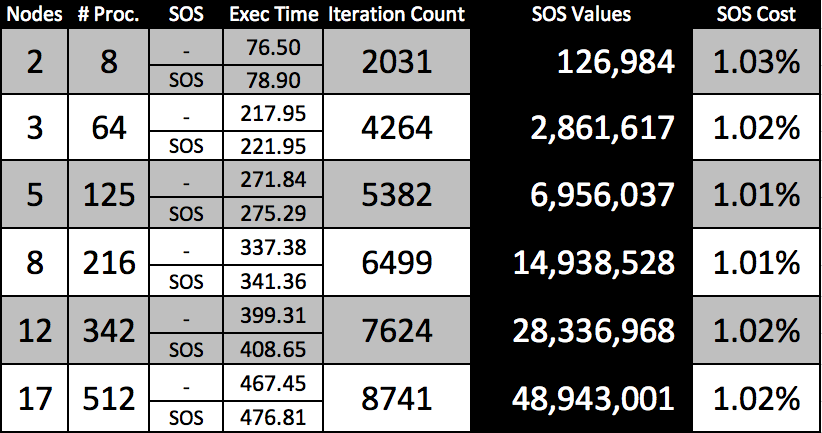
\includegraphics[width=5in]{images/cori_results.png}
\caption{Impact of SOSflow on LULESH Experiments}
\label{cori_results}
\end{figure*}
%%%%%

%\todofileend{040\_evaluation\_validation.tex}
